\begin{frame}[fragile]{Making Milestoning Practical: Transition-Path Theory and \\ Markovian Milestoning in Voronoi Tesselations}
\begin{tikzpicture}[scaleall=1.0]
\pcuad{\textwidth}{\textheight}
%\showcuad
\path(nw) ++(-0.75,0.15) node(text)[anchor=north west,text 
width=\textwidth]{{\tiny \textcolor{red!80!black}{
E. Vanden-Eijnden et al. {\it J Chem Phys} {\bf 130}:194101 (2009).}}};
\path(nw) ++(-0.75,-0.5) node(text2)[anchor=north west,text width=1.1\textwidth]{
Estimate \textcolor{blue}{$\ds q_{ik,ij}$} using MD confined to Voronoi cells in feature-space};
\path(nw) ++(-0.75,-1.5) node(image1)[anchor=north west]{
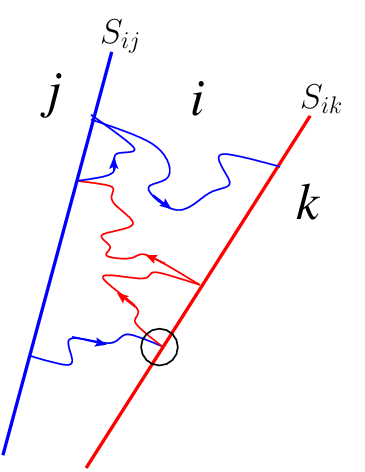
\includegraphics[width=0.4\textwidth]{milestoning2}};
\path(nw) ++(4.25,-1.0) node(text3)[scale=0.7,anchor=north west,text width=0.8\textwidth]{
In each cell $i$, use confined MD of duration $T_i$ to tally:
\begin{enumerate}
\item $N^i_{ik,ij}$,
\item $R^i_{ij}$,\ and,
\item $N^i_{i\rightarrow j}$: \# of transition attemps from $i$ to any neighbor $j$.
\end{enumerate}
Compute apparent transition rate constants:
\begin{displaymath}
k_{i\rightarrow j} = \frac{\ds N^i_{i\rightarrow j}}{\ds T_i}
\end{displaymath}
And enforce equilibrium among all $\Lambda$ cells, so
\begin{displaymath}
\sum_{j=1,j\ne i}^{\Lambda} \pi_j k_{j\rightarrow i} = \pi_i\sum_{j=1;j\ne i}^{\Lambda} k_{i\rightarrow j}\ \ \sum_i\pi_i = 1
\end{displaymath}
providing equilibrium probabilities to be in cell $i$, $\pi_i$.  This allows construction of $q_{ik,ij}$:
\begin{displaymath}
q_{ik,ij} = \frac{\ds \pi_i N^i_{ik,ij}/T_i}{\ds \pi_i R^i_{ij}/T_i + \pi_j R_{ij}^j/T_j}.
\end{displaymath}
};
\end{tikzpicture}
\end{frame}

